\section{Shortcomings of Application Parallelism}

Several recent works~\cite{Esmaeilzadeh2011Dark-silicon-an,Hardavellas:2011de}
have looked at the impact of dark silicon on computing in the near future. While
the number of transistors on a given die have been doubling every generation,
the number of transistors that can be powered for a fixed power budget have not
been increasing due to the slowing of transistor performance scaling. Since
power budgets have not been increasing past the limits defined by air cooling,
this has led to a situation where chips have more transistors than can be
powered at any given time. These unpowered transistors are referred to as dark
silicon.

Dark silicon seemingly presents an opportunity for near-threshold computing.
Deslinkski et al.~\cite{dreslinski2010near} state . ``More gates can now fit on
a die, but a growing fraction cannot actually be used due to strict power
limits.'' By reducing the power consumed per-core, more cores can be integrated
and simultaneously powered. Since these cores would be unpowered in a
super-threshold chip, this represents an opportunity for near-threshold chips to
regain performance compared to super-threshold operation.

\begin{figure}[thpb]
    \centering
    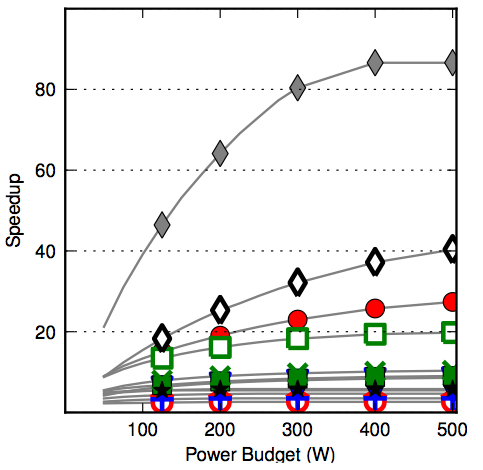
\includegraphics[width=0.3\textwidth]{esmaeilzadeh_power_speedups.png}
    \caption{Project speedups on PARSEC benchmarks while the chip power
constraint (and therefore number of cores) is unconstrained. ~\cite{Esmaeilzadeh2011Dark-silicon-an}}
    \label{fig:power_speedups}
\end{figure}

While this dark silicon is an opportunity for devices to reach higher levels of
integration, recent studies analyzing dark silicon have not born out the
promise of higher levels of performance with increasing core counts.  Work by
Esmaeilzadeh et. al~\cite{Esmaeilzadeh2011Dark-silicon-an} developed an
analytical model analyzing the impact of dark silicon for a range of CMP
configurations in future process technologies. They show projected speedups for
these configurations and process technologies using the PARSEC benchmark suite,
which represents workloads similar to the SPLASH2 benchmark suite used in the
previously discussed clustering architecture
papers~\cite{dreslinski2010near,Zhai:2007kn}, indicating that they are
targeting similar applications. This analytical model does project that dark
silicon will become a significant portion of CPUs in the near future,
dominating as soon as 2016 assuming conservative scaling parameters. However,
the authors also analyze the case where the power constraint is lifted, which
effectively removes the impact of dark silicon and allows more cores to be
powered. Figure~\ref{fig:power_speedups} shows the projected speedups on
different PARSEC benchmarks as the power constraint is increased. Increasing
the power constraint reduces the effect of dark silicon as more cores can
simultaneously be powered. The paper projects that if the amount of parallelism
in applications were increased to 99\%, then the best case speedup for power
limited cores in \SI{8}{\nano\meter} is 15x relative to a quad-core Nehalem
processor at \SI{45}{\nano\meter}. However, as shown in
figure~\ref{fig:power_speedups}, with an unconstrained power budget, and the
same current amount of application level parallelism, 8 out of 12 PARSEC
benchmarks achieve no more than 10x speedup. What this indicates is that the
amount of parallelism in general-purpose parallel workloads is currently not
exploitable even by future power constrained multi-core chips. While
near-threshold computing would allow more chips to be powered, it would not
realize a significant speedup on most general-purpose parallel workloads due to
the lack of exploitable parallelism.

\begin{figure}[thpb]
    \centering
    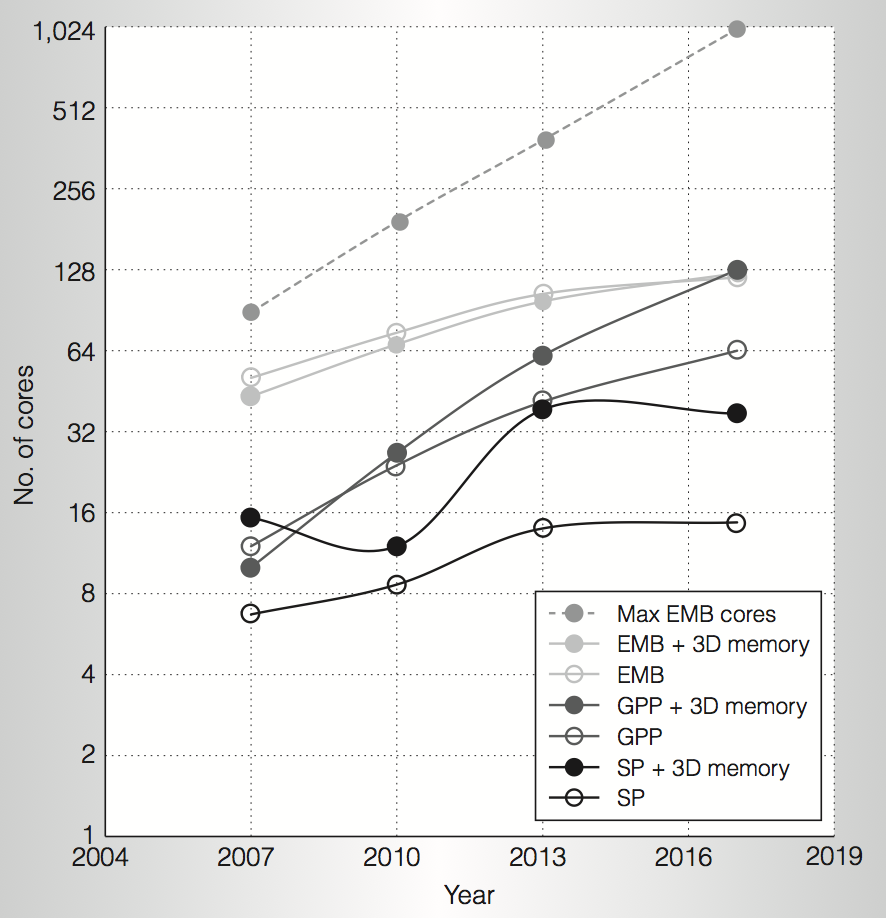
\includegraphics[width=0.4\textwidth]{hardavellas_core_counts.png}
    \caption{Projections for core count scaling.~\cite{Hardavellas:2011de}}
    \label{fig:core_counts}
\end{figure}

\begin{figure}[thpb]
    \centering
    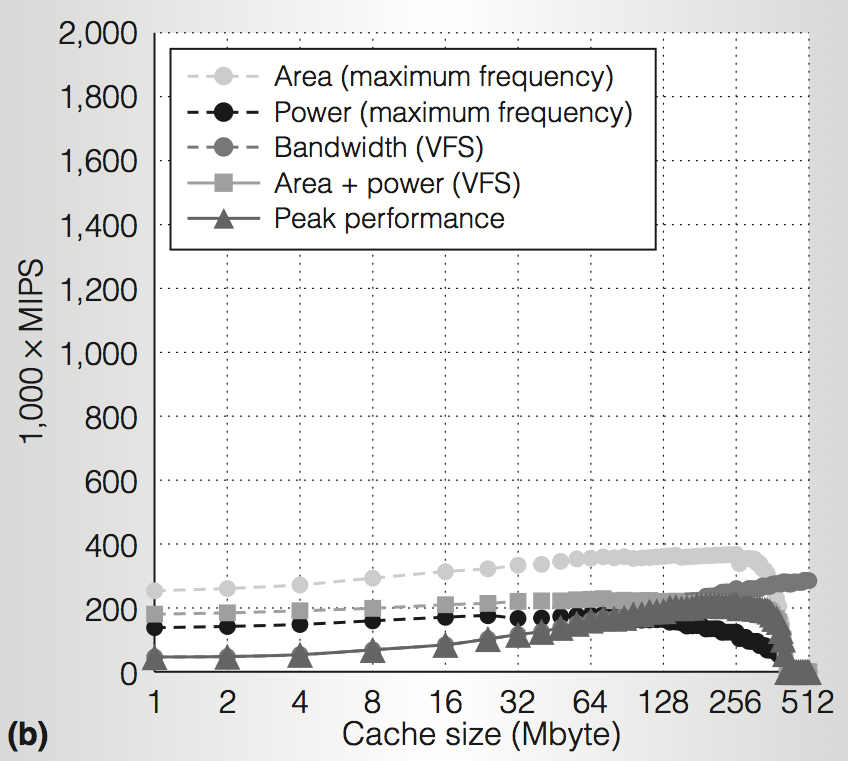
\includegraphics[width=0.4\textwidth]{hardavellas_emb_performance.png}
    \caption{Embedded core scaling.~\cite{Hardavellas:2011de}}
    \label{fig:emb_performance}
\end{figure}

Further work by Hardavellas et al.~\cite{Hardavellas:2011de} confirms this
observation that future speedups are limited by application level parallelism,
not power constraints. Figure~\ref{fig:core_counts} shows projected core count
scaling trends in future process technologies. The key lines to focus on are
``EMB cores'' and ``Max EMB cores'', where EMB represents a low-power embedded
core similar to an ARM11 MPCore. The EMB line represents how many cores can be
built without increasing power or die size constraints, where the Max EMB cores
line represents the maximum number of cores that could fit on the same die
area. It is project that in 2017 over 1024 cores will be able to fit on a die,
but only 12\% of them will be able to be powered at any given time. This again
looks like an opportunity for near-threshold computing to take advantage of
being able to power a larger number of cores simultaneously.

Figure~\ref{fig:emb_performance} shows the maximum performance of an EMB-based
CMP given different constraints. The ``Area (maximum frequency'' line
represents the best performance with only a die area constraint, while the
``Peak Performance'' line represents the best performance factoring in area,
power, and memory bandwidth constraints.

